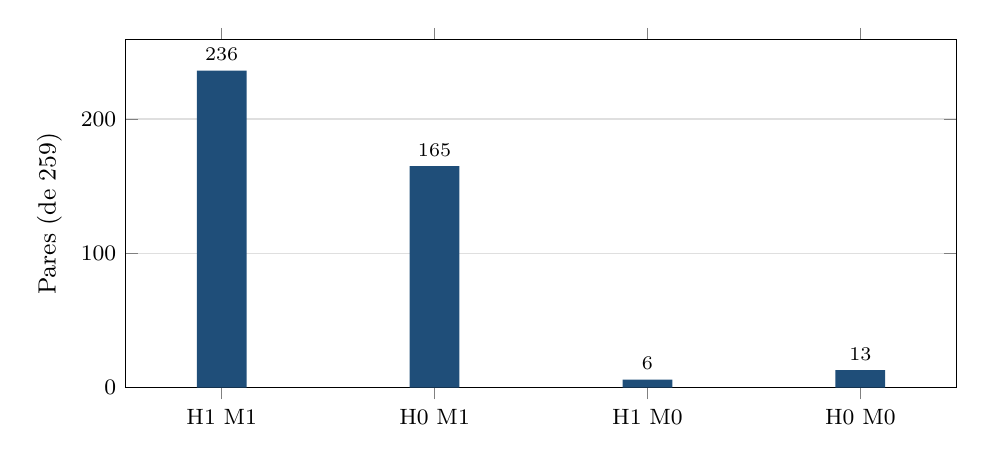
\begin{tikzpicture}
\begin{axis}[
  ybar,
  bar width=18pt,
  width=\linewidth,
  height=6cm,
  xtick={0,...,3},
  xticklabels={{H1 M1},{H0 M1},{H1 M0},{H0 M0}},
  ylabel={Pares (de 259)},
  /pgf/number format/use comma,
  /pgf/number format/precision=0,
  /pgf/number format/fixed,
  ymajorgrids,
  grid style={gray!25},
  enlarge x limits=0.15,
  tick label style={font=\footnotesize},
  label style={font=\small},
  ymin=0,
  ymax=259,
  nodes near coords,
  every node near coord/.append style={font=\scriptsize}
]
\addplot[fill={rgb,255:red,31;green,78;blue,121}, draw=none] coordinates {(0,236.0000) (1,165.0000) (2,6.0000) (3,13.0000)};
\end{axis}
\end{tikzpicture}
